\documentclass[11pt,a4paper]{article}

%% ── Packages ─────────────────────────────────────────────────────────────────
\usepackage[T1]{fontenc}
\usepackage[utf8]{inputenc}
\usepackage[top=2.6cm,bottom=2.6cm,left=2.7cm,right=2.7cm]{geometry}
\usepackage{setspace}
\usepackage{titlesec}
\usepackage{amsmath,amssymb}
\usepackage{booktabs}
\usepackage{array}
\usepackage{graphicx}
\usepackage{float}
\usepackage{caption}
\usepackage[dvipsnames]{xcolor}
\usepackage{hyperref}
\usepackage{enumitem}
\usepackage[numbers,sort&compress]{natbib}
\usepackage{fancyhdr}
\usepackage{amsthm}

%% ── Hyperref ──────────────────────────────────────────────────────────────────
\hypersetup{colorlinks=true,linkcolor=NavyBlue,citecolor=NavyBlue,urlcolor=NavyBlue}

%% ── Section headings ─────────────────────────────────────────────────────────
\titleformat{\section}{\large\bfseries}{\thesection}{0.7em}{}
\titleformat{\subsection}{\normalsize\bfseries}{\thesubsection}{0.6em}{}
\titlespacing*{\section}{0pt}{15pt}{6pt}
\titlespacing*{\subsection}{0pt}{11pt}{4pt}

%% ── Spacing ───────────────────────────────────────────────────────────────────
\setstretch{1.12}
\setlength{\parindent}{1.4em}
\setlength{\parskip}{0pt}

%% ── Captions ─────────────────────────────────────────────────────────────────
\captionsetup{font=small,labelfont=bf,labelsep=period,skip=7pt,width=0.95\textwidth}

%% ── Theorem-like environments ────────────────────────────────────────────────
\theoremstyle{definition}
\newtheorem{definition}{Definition}

%% ── Custom ────────────────────────────────────────────────────────────────────
\newcommand{\MCR}{\ensuremath{\mathrm{MCR}}}

%% ─────────────────────────────────────────────────────────────────────────────
\begin{document}
%% ─────────────────────────────────────────────────────────────────────────────

\begin{titlepage}
\thispagestyle{empty}
\vspace*{2.0cm}
\begin{center}
  {\LARGE\bfseries The Mean-Crossing Rate of the Price Ratio\\[7pt]
   as a Pair-Selection Criterion\par}
  \vspace{12pt}
  {\large Arnav Rayaprolu$^{\dagger}$ \& Sudeep R. Bapat$^{*}$}
  \vspace{10pt}
  \vspace{7pt}\\
  {\normalsize $^{\dagger}$Oberoi International School, India \par}
  \vspace{4pt}
  {\normalsize $^{*}$Shailesh J. Mehta School of Management, Indian Institute of Technology Bombay, India \par}
    \vspace{7pt}
  {\normalsize Email: $^{*}$sudeepb@iitb.ac.in \par}
\end{center}
\vspace{5pt}
\begin{center}
\begin{minipage}{0.90\textwidth}
\setstretch{1.05}

\vspace{2pt}
\small
\begin{abstract}
Pairs trading relies on selecting securities that exhibit a stable relation-
ship, but conventional criteria such as cointegration, correlation, and price-path
distance do not directly measure how frequently that relationship returns to
equilibrium. We introduce the Mean-Crossing Rate (MCR), a non-parametric
pair-selection criterion measuring the frequency with which the moving-average
z-score of the price ratio crosses zero. We also propose hybrid criteria combining
MCR with conventional measures through rank aggregation.
Seven criteria are evaluated on S\&P 500 constituents using two years
of hourly data and a nine-fold non-overlapping walk-forward design. The
MCR+Cointegration hybrid returns 48.2\% net of 3 bps round-trip transaction
costs, with a Sharpe ratio of 2.02, compared with 13.5\% and 0.72 for cointegration alone. MCR alone returns 7.9\%, outperforming distance and correla-
tion. Two of three pre-specified Diebold–Mariano comparisons are significant
after Holm correction, although significance does not survive correction for the
broader specification search. Overall, the results suggest that oscillation fre-
quency provides useful complementary information to structural measures of
long-run equilibrium in pair selection.
\end{abstract}


\vspace{8pt}
\noindent\textbf{Keywords:} Pairs Trading; Mean-Crossing Rate; Pair Selection;
Statistical Arbitrage; Cointegration; Diebold--Mariano Test; Walk-Forward
Validation; S\&P~500.
\end{minipage}
\end{center}
\vfill
\end{titlepage}

\setcounter{page}{1}

%% ─────────────────────────────────────────────────────────────────────────────
\section{Introduction}
%% ─────────────────────────────────────────────────────────────────────────────

Pairs trading buys the cheap leg and shorts the expensive leg of two related
securities that have diverged, closing both when the gap narrows. The two legs
offset directional exposure, leaving a position that is close to market neutral.
Since the empirical study of \citet{gatev2006} it has been the canonical
statistical arbitrage strategy, and it sits within a broader literature on
relative-value trading in equities~\citep{avellaneda2010}.

Selection is the strategy's principal design choice. With the trading engine
held fixed, the only thing that varies across methods is which pairs are traded,
so differences in realised performance measure selection quality directly. This
is the experimental design used throughout.

The criteria in standard use are structural. Cointegration tests whether a
linear combination of two price series is stationary. Correlation tests whether
returns co-move. Distance tests whether normalised price paths tracked closely.
Each answers a question about the existence of a relationship. None
answers a question about its \emph{tempo}: how often the relationship actually
passes back through equilibrium. Tempo is what makes a relationship tradable at
short horizons. A pair that is unimpeachably cointegrated but reverts over
months cannot be traded profitably inside a 45-day window, however strong its
test statistic.

This paper introduces the Mean-Crossing Rate as a criterion for that missing
property, and a hybrid criterion that combines it with a structural measure. Two
construction choices are fixed throughout. The object of study is the
price ratio $r_t = P^A_t/P^B_t$ rather than an OLS-hedged spread, so no
hedge ratio has to be estimated and the statistic corresponds exactly to the
equal-dollar position the engine takes. The $z$-score uses the
moving-average difference form, which determines what a zero-crossing
represents. Unlike existing selection criteria that certify the existence of a long-run equilibrium,
the proposed criterion is motivated by the observation that, over a fixed investment
horizon, expected cumulative trading profits depend not only on the existence of
mean reversion but also on the frequency with which mean-reversion opportunities occur.
Section~\ref{sec:theory} formalises this intuition.

The remainder of the paper is organised as follows. Section~\ref{sec:lit}
reviews the selection literature and locates the gap. Section~\ref{sec:method}
defines \MCR, the hybrid criterion, the trading engine and the capital rule.
Section~\ref{sec:theory} establishes what the statistic measures.
Section~\ref{sec:data} describes the data and walk-forward design.
Section~\ref{sec:results} reports performance, the three Diebold--Mariano tests
and cost sensitivity. Sections~\ref{sec:limits} and~\ref{sec:conc} discuss
limitations and conclusions.

%% ─────────────────────────────────────────────────────────────────────────────
\section{Literature Review}
\label{sec:lit}
%% ─────────────────────────────────────────────────────────────────────────────
This section reviews the main approaches to pair selection in statistical
arbitrage and positions the proposed MCR criterion within this literature.
We first discuss established selection criteria and their declining empirical
performance, before considering mean-reversion speed, crossing-rate methods,
and composite selection criteria.

\subsection{Selection Criteria}

The modern literature begins with \citet{gatev2006}, which presents a pair-selection
technique based on the minimum sum of squared deviations between normalised price
paths over a twelve-month formation window, and trades divergences beyond two
historical standard deviations. On US equities from 1962 to 2002 the rule earned
annualised excess returns of roughly $11\%$. Its advantage is that it is entirely
non-parametric: no model of the spread is estimated, and the criterion is a
simple distance.

The main alternative replaces distance with a formal test for a stable long-run
relationship. \citet{engle1987} established the cointegration framework, and
\citet{vidyamurthy2004} adapted it to pairs trading: two price series that are
individually integrated may admit a stationary linear combination, and that
combination is the spread to trade. Cointegration is theoretically more
satisfying than distance because stationarity of the spread is precisely the
property mean-reversion trading requires. \citet{elliott2005} takes a step further,
modelling the spread explicitly as a mean-reverting Gaussian state process
and filtering it, which yields both an estimate of the equilibrium level and a
measure of how quickly the spread returns to it.

A third family selects on return correlation, and a fourth on copulas, which
capture dependence beyond the linear case. \citet{rad2016} compares distance,
cointegration and copula selection on a common US sample and finds that the
distance and cointegration methods perform comparably, while the copula approach
does not drastically improve on either. \citet{huck2015} poses the question directly, whether cointegration is superior, and concludes that the answer depends
on the market and period rather than holding generally.

\subsection{Declining Performance and the Case for New Criteria}

\citet{do2010} document a substantial decline in distance-method profitability
in the decades after the \citet{gatev2006} sample, attributing it partly to
increased competition and partly to a genuine reduction in the frequency with
which pairs converge. \citet{krauss2017} surveys the field and reaches a similar
conclusion: the classical criteria are well understood, widely implemented, and
their edge has compressed. This motivates the search for selection criteria that
capture properties the established measures do not.

The established selection criteria all measure structural properties of the
\emph{level} relationship between two price series and its stability. None
measures the frequency with which the relationship revisits equilibrium. This
distinction is particularly important at intraday and hourly horizons, where
strategy performance depends on the number of completed mean-reversion
opportunities within the trading window rather than simply on the existence of a
long-run equilibrium.

\subsection{Speed of Mean Reversion}

The literature does contain a notion of mean reversion speed, usually through the
Ornstein--Uhlenbeck process. \citet{vasicek1977} introduced the model in a
term-structure setting; applied to a pair spread, it yields a reversion parameter
$\kappa$ and an implied half-life of $\ln 2/\kappa$. \citet{bertram2010} derives
analytic optimal entry and exit thresholds for a spread following this process,
making the dependence of expected profit on $\kappa$ explicit. Consequently,
estimated half-life is often used as a screening criterion, with pairs exhibiting
excessively slow reversion discarded before portfolio construction.

Half-life, however, is a screening filter rather than a selection criterion. It
estimates the expected time required for a deviation to decay by one half under a
parametric stochastic model, but it does not quantify how frequently trading
opportunities arise over a finite investment horizon. Further, its estimation
relies on the assumptions of the OU process, including a constant mean-reversion
speed, Gaussian innovations, and a fixed equilibrium level. The proposed
Mean-Crossing Rate (MCR) is entirely non-parametric. Rather than estimating a
model of the spread, it measures the empirical frequency with which the observed
trading signal revisits equilibrium and uses this frequency to rank all candidate
pairs.

\subsection{Crossing Rates}

Counting the crossings of a level is a classical technique in signal processing
rather than finance. \citet{rice1944} derived the expected zero-crossing rate of
a stationary Gaussian process, showing it is determined by the spectral moments
of the process. For a standardised Ornstein--Uhlenbeck process the rate is
$\kappa/\pi$, linking crossing frequency directly to reversion speed.
\citet{vanvleck1966} established the arcsine law relating the probability of a
sign change between consecutive samples to the lag-one autocorrelation, and
\citet{kedem1986} developed zero-crossing counts into a practical tool for
spectral discrimination, showing they carry substantial information about a
process at very low computational cost.

These results supply the theoretical basis for using a crossing count as a
measure of oscillation frequency. To our knowledge they have not been applied as
a pair-selection criterion in the pairs-trading literature, where crossing
behaviour is normally treated as an output of the trading rule rather than an
input to selection.

\subsection{Composite Criteria and Inference}

\citet{reichmann2026} argues that pair selection is better treated as a scoring
problem than as a single-criterion ranking, and finds that composite scores
constructed from several inputs produce more competitive returns than any
component alone. This motivates the hybrid criterion developed here, which
aggregates the ranks of a frequency measure and a structural measure.

From the statistical inference side, comparisons between trading rules are
naturally framed as tests of equal predictive accuracy. \citet{diebold1995} gives
the standard test, which examines whether two competing forecasting methods have
equal predictive accuracy; \citet{harvey1997} provides a small-sample correction to
it, and \citet{newey1987} gives the heteroskedasticity- and
autocorrelation-consistent variance estimator required at high frequency. Because
backtest comparisons involve searching over specifications, \citet{white2000} and
\citet{lopezdeprado2018} suggests correcting for the size of that search, and
\citet{bailey2014} proposes a Sharpe ratio deflated for both selection intensity
and non-normality. We follow this literature by pre-specifying the hypotheses
tested and reporting multiplicity corrections at two scopes.

%% ─────────────────────────────────────────────────────────────────────────────
\section{Methodology}
\label{sec:method}
%% ─────────────────────────────────────────────────────────────────────────────

The empirical framework is designed to isolate the effect of pair selection from the subsequent trading rule. In each formation window, all candidate pairs are evaluated using the proposed Mean-Crossing Rate (MCR), three established selection criteria, and their corresponding MCR-based hybrids. Each criterion is then used to select a fixed number of pairs, which are traded over the subsequent out-of-sample window using an identical signal, capital-allocation rule, and transaction-cost specification. The differences in realised performance across portfolios can be attributed primarily to the pair-selection criterion rather than to differences in trading implementation. Figure~\ref{fig:method} presents a flowchart that summarises the complete procedure.


\begin{figure}[H]
\centering
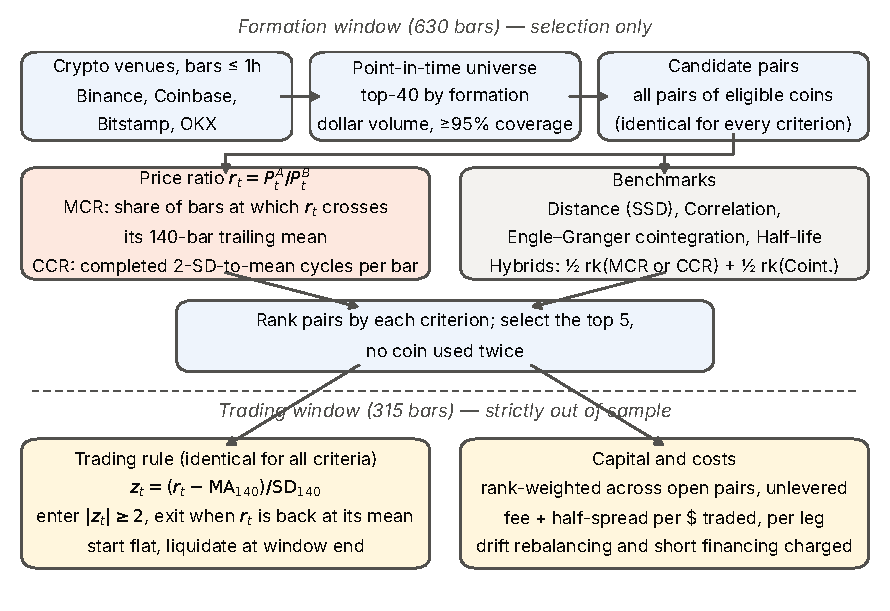
\includegraphics[width=\textwidth]{figures/fig_methodology.pdf}
\caption{The pipeline. Everything above the division uses the training window
only; everything below is applied out of sample. All four statistics are
computed on the same candidate set, and one engine and cost model are applied to
every criterion.}
\label{fig:method}
\end{figure}

\subsection{The Signal}

For an ordered pair $(A,B)$ define the price ratio $r_t$ and its $z$-score $z_t$ as,
\begin{align}
  r_t &\;=\; \frac{P^A_t}{P^B_t}, \label{eq:ratio}\\[4pt]
  z_t &\;=\;
  \frac{\mathrm{MA}_f(r)_t - \mathrm{MA}_s(r)_t}{\mathrm{SD}_s(r)_t},
  \label{eq:z}
\end{align}
where $\mathrm{MA}_w$ and $\mathrm{SD}_w$ are the trailing $w$-bar mean and
standard deviation, which take the following form

\begin{equation}
    \operatorname{MA}_{w}(r)_t
    = \frac{1}{w}\sum_{j=0}^{w-1} r_{t-j},
    \label{eq:ma}
\end{equation}
and
\begin{equation}
    \operatorname{SD}_{w}(r)_t
    =
    \left[
    \frac{1}{w-1}
    \sum_{j=0}^{w-1}
    \left(r_{t-j}-\operatorname{MA}_{w}(r)_t\right)^2
    \right]^{1/2}.
    \label{eq:sd}
\end{equation}
Thus, both quantities are computed using only the current and preceding
$w-1$ observations. Here, $f = 35$ bars (5 trading days) and $s = 140$ bars (20
trading days) at hourly resolution. Every window is backward-looking and
terminates at $t$, so $z_t$ is observable at $t$.

Working on the ratio rather than a hedged spread has two consequences. No
regression is required, so the signal carries no hedge-ratio estimation error
and cannot be destabilised by a poorly identified $\hat{\beta}$. Moreover, the ratio
maps exactly onto an equal-dollar long/short position, which is the position the
engine takes, so the quantity ranked and the quantity traded are the same
object.

\subsection{The Mean-Crossing Rate}

For a candidate pair $(A,B)$, let $z_1,\ldots,z_T$ denote the z-score
series observed over a formation window of $T$ bars. The empirical
Mean-Crossing Rate (MCR) is defined as
\begin{equation}
  \widehat{\MCR}_{AB} \;=\; \frac{1}{T}
  \sum_{t=2}^{T}\mathbf{1}\!\left[\,\mathrm{sgn}(z_t)\neq\mathrm{sgn}(z_{t-1})\,\right],
  \label{eq:mcr}
\end{equation}
where $\mathbf{1}\{\cdot\}$ denotes the indicator function. Observations
for which $z_t=0$ are excluded when determining consecutive sign changes.

Thus, $\widehat{\mathrm{MCR}}_{AB}$ is the observed proportion of
consecutive formation-period observations for which the trading signal
changes sign. A larger value indicates that the standardised price-ratio
signal crosses its equilibrium more frequently and therefore exhibits a
higher empirical oscillation frequency.


Pairs are ranked in descending $\widehat{\MCR}$: the criterion prefers pairs
whose standardised ratio passes back through its equilibrium often. The measure
is non-parametric, requires no distributional assumption, and can be computed in a single pass over the series.

Further, no filters are applied: there are no stationarity checks, no half-life
ceiling, and no hedge-ratio quality gate. Earlier versions of this study included
an Ornstein--Uhlenbeck half-life gate and a Hurst exponent screen. Both were
removed after they were found not to change the selected pairs of any hybrid in
any fold, so the reported results carry no tuning associated with them.

\subsection{Benchmark Criteria}

To evaluate whether MCR provides information beyond conventional pair-selection methods, three established criteria---cointegration, distance, and return correlation---are computed on an identical formation window and on the same set of candidate pairs. For the \emph{cointegration criterion}, the Engle--Granger two-step procedure \citep{engle1987, vidyamurthy2004} is applied to the logarithmic price series of each pair. The residual series from the cointegrating regression is tested for stationarity using an augmented Dickey--Fuller test \citep{dickey1979}. Candidate pairs are ranked in ascending order of the resulting ADF $p$-value, so that stronger evidence of cointegration corresponds to a higher selection priority. For the \emph{distance criterion}, following \citet{gatev2006}, each price series is normalised by its value at the beginning of the formation window. The distance between stocks $A$ and $B$ is then measured by the sum of squared deviations, as given by
\begin{equation} \operatorname{SSD}_{AB} = \sum_{t=1}^{T} \left( \frac{P_t^A}{P_1^A} - \frac{P_t^B}{P_1^B} \right)^2.
\label{eq:ssd}
\end{equation}
Pairs with smaller values of $\operatorname{SSD}_{AB}$ exhibit more similar normalised price paths and are therefore ranked higher.

Finally, the \emph{correlation criterion} measures the Pearson correlation between the hourly log returns of the two securities over the formation window. Pairs are ranked in descending order of correlation, with larger positive correlations indicating stronger short-horizon co-movement.

\subsection{The Hybrid Criterion}

The hybrid criterion combines MCR with each benchmark criterion, reflecting the
idea that oscillation frequency and structural similarity provide complementary
information for pair selection. Following \citet{reichmann2026}, the hybrid score
is defined as an equally weighted average of percentile ranks,
\begin{equation}
\Phi_{AB}^{(m)}
=
\frac{1}{2}\operatorname{rk}(\widehat{\mathrm{MCR}}_{AB})
+
\frac{1}{2}\operatorname{rk}(C_{AB}^{(m)}),
\label{eq:hybrid}
\end{equation}
where $C_{AB}^{(m)}$ denotes the value of benchmark criterion $m$ for pair
$(A,B)$, with $m$ being either Cointegration, Distance, or Correlation, and $\operatorname{rk}(\cdot)\in[0,1]$ denotes the corresponding percentile rank,
oriented so that larger values are always preferred. Percentile ranks place the two components on a common scale and
prevent either criterion from dominating the blend through its units.

The design intent is that the two components certify different things. A
structural criterion certifies that an equilibrium relationship exists, while \MCR{}
certifies that the spread returns to it often enough to be traded. Averaging
ranks favours pairs that score well on both, rather than pairs that score
extremely on one and poorly on the other.

Candidate pairs are restricted to combinations of stocks belonging to the same Global Industry Classification Standard (GICS) sector. This restriction
is economically motivated, since firms within the same sector are more likely to share
common risk factors that support convergence, and is also computationally convenient,
reducing roughly 125,000 unordered combinations to about 13,000 per fold. From the
resulting ranked list, the top five pairs are selected subject to the constraint that no
ticker appears in more than one pair, thereby avoiding excessive concentration in a
single stock through overlapping pairs.

\subsection{Trading Engine}

The engine is minimal and identical across all seven criteria:
\begin{itemize}[leftmargin=1.6em,itemsep=2pt,topsep=3pt]
  \item $z_t \le -1.00$: buy the ratio (long $A$, short $B$).
  \item $z_t \ge +1.00$: sell the ratio (short $A$, long $B$).
  \item Exit when $|z_t| \le 0.25$. No stop-loss and no maximum holding period.
\end{itemize}

The position implied by $z_t$ is held over bar $t+1$ and earns bar $t+1$'s
return, so no contemporaneous information enters the return. Each leg receives
half the capital allocated to the pair, so a unit position earns
$\pi_t = \tfrac{1}{2}(r^A_t - r^B_t)$ and is dollar neutral by construction. Figure~\ref{fig:legs} illustrates how the sign of the z-score determines the direction of the
pair trade. When $z_t\leq-1$, the ratio is bought by taking a long position in
stock $A$ and a short position in stock $B$; when $z_t\geq1$, the positions are
reversed.

Figure~\ref{fig:signal} provides an example of the trading rule for the ADP/WM pair over one
out-of-sample window. Positions are initiated when the z-score enters the
pre-specified entry region and are closed as it returns to the exit region around
zero. The figure illustrates how repeated oscillations of the ratio signal generate
multiple entry--exit opportunities, which is the behaviour that MCR is designed
to capture.

\begin{figure}[H]
\centering
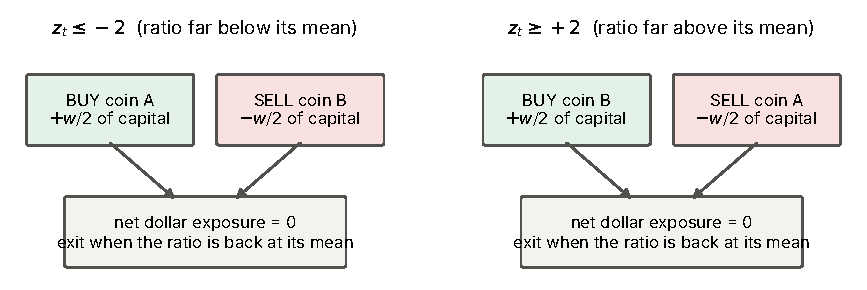
\includegraphics[width=\textwidth]{figures/fig_legs.pdf}
\caption{Leg assignment. The sign of $z$ determines which ticker is bought and
which is sold; each receives half the capital allocated to the pair, so the
position carries no net dollar exposure.}
\label{fig:legs}
\end{figure}

\begin{figure}[H]
\centering
\includegraphics[width=\textwidth]{figures/fig_signal.pdf}
\caption{Ratio $z$-score for one selected pair over its out-of-sample fold. Red
bands mark the entry zone $1.00 \le |z| \le 1.25$, the green band the exit zone
$|z| \le 0.25$; markers indicate realised position changes.}
\label{fig:signal}
\end{figure}

\subsection{Capital Deployment}

A pair holds a position only while $|z|$ has breached the entry threshold and
has not yet reverted, so only a subset of the five selected pairs is active at
any bar. Capital is allocated across that active subset, weighted by selection
rank. Let $\mathcal{A}_t$ denote the set of pairs that are active at bar $t$, and let
$\operatorname{pos}_{i,t}\in\{-1,0,1\}$ denote the trading position in pair $i$,
with the sign indicating the direction of the ratio trade. Let $\Phi_i$ denote
the formation-period selection score of pair $i$. The signed portfolio weight
assigned to pair $i$ at time $t$ is then

\begin{equation}
W_{i,t}
=
\operatorname{pos}_{i,t}
\frac{\Phi_i\,\mathbf{1}\{i\in\mathcal{A}_t\}}
{\sum_j \Phi_j\,\mathbf{1}\{j\in\mathcal{A}_t\}},
\label{eq:weights}
\end{equation}
with $W_{i,t} = 0$ for all $i$ when $\mathcal{A}_t$ is empty. Since membership of
$\mathcal{A}_t$ follows from $z_{t-1}$, and $\Phi_i$ is a formation-window
quantity, $W_{i,t}$ is known before bar $t$'s return is realised. Portfolio gross
return and turnover are given as
\begin{equation}
  g_t \;=\; \sum_i W_{i,t}\,\pi_{i,t},
  \qquad
  u_t \;=\; \sum_i \left|W_{i,t} - W_{i,t-1}\right|,
  \label{eq:pgross}
\end{equation}
and net return is $n_t = g_t - u_t\,c/2$, where $c$ denotes the round-trip transaction cost, set to
$3$~bps throughout. The factor $c/2$ accounts for the fact that a complete round trip consists of both opening and closing a position. Thus, the cumulative turnover associated with a unit position over its full holding period is two, resulting in a total transaction cost of $c$.

Turnover is computed from changes in the portfolio weights rather than solely from position entries and exits. This is important because changes in the set of active pairs may require existing positions to be resized, generating additional trading costs. The resulting cost specification therefore accounts for both position changes and portfolio rebalancing. All reported results are net of these transaction costs.

%% ─────────────────────────────────────────────────────────────────────────────
\section{Statistical Interpretation of the Mean-Crossing Rate}
\label{sec:theory}
%% ─────────────────────────────────────────────────────────────────────────────

Crossing counts are conventionally justified through level-crossing theory.
\citet{rice1944} gives the expected zero-crossing rate of a stationary Gaussian
process. For a standardised Ornstein--Uhlenbeck process~\citep{vasicek1977}
with reversion speed $\kappa$, that rate is $\kappa/\pi$, so crossing frequency
is proportional to reversion speed.

That identity requires care in the present setting. From
Equation~\eqref{eq:z},
\begin{equation}
  z_t = 0 \quad\Longleftrightarrow\quad \mathrm{MA}_f(r)_t = \mathrm{MA}_s(r)_t.
  \label{eq:crossmeaning}
\end{equation}
Thus, a zero-crossing of $z_t$ corresponds to a crossover between the fast and
slow moving averages of the price ratio, rather than to the ratio itself crossing
its mean. Consequently, MCR measures the crossing frequency of a filtered version
of the price ratio. While Rice's general level-crossing framework remains applicable
to such a process, the specific $\kappa/\pi$ relationship for an
Ornstein--Uhlenbeck process does not apply directly.

A more precise characterisation follows from the relationship between sign changes
and serial dependence. For a zero-mean stationary Gaussian process with lag-one
autocorrelation $\rho_1$, the probability that two consecutive observations have
different signs is
\begin{equation}
\Pr\!\left[\operatorname{sgn}(z_t)\neq\operatorname{sgn}(z_{t-1})\right]
=
\frac{\arccos(\rho_1)}{\pi},
\label{eq:kedem}
\end{equation}
a result due to the arcsine law of \citet{vanvleck1966} and subsequently used in
zero-crossing-based spectral analysis by \citet{kedem1986}. $\widehat{\MCR}$ is
therefore the sample analogue of this crossing probability when applied to the
filtered ratio signal. Since the expression is decreasing in $\rho_1$, a higher
MCR corresponds to lower persistence and more frequent oscillations of the signal
around zero. We verified
Equation~\eqref{eq:kedem} numerically on simulated AR(1) processes, where for
$\phi \in [0.80, 0.99]$, the implied rate matched the realised crossing rate to
within $0.0015$.

One practical consequence of the moving-average difference form is that $z$ is
strongly compressed. Differencing two moving averages of the same series removes
the low-frequency component that dominates the ratio's variance, so the
numerator of Equation~\eqref{eq:z} is small relative to the denominator.
Empirically, $|z|$ rarely exceeds $1.7$, whereas the textbook standardisation
$(r_t - \mathrm{MA})/\mathrm{SD}$ routinely exceeds $5$ on the same data. Entry
at $|z| = 1.00$ is therefore a considerably more conservative rule than the
numeric threshold suggests.

\subsection{Economic Interpretation of the Mean-Crossing Rate}

The Mean-Crossing Rate is intended as a proxy for the frequency with which a trading opportunity completes a full entry--exit cycle. Suppose that a completed round-trip trade generates a random profit $G$ with
finite expectation $\mu_G=E(G)$, and let $N(T)$ denote the number of completed
mean-reversion cycles during a trading horizon of length $T$. Let $R(T)$ denote
the cumulative trading profit over this horizon. Ignoring transaction costs for
the moment,

\begin{equation}
R(T)=\sum_{i=1}^{N(T)} G_i,
\end{equation}
where $\{G_i\}$ are the realised profits from successive completed trades. Taking expectations gives \begin{equation}
E[R(T)] = E[N(T)]\,E[G],
\end{equation}
provided that the average profit per completed cycle is stable over the trading horizon. Since the Mean-Crossing Rate estimates the average number of equilibrium crossings per observation,
\begin{equation}
E[N(T)] \approx T \times \mathrm{MCR},
\end{equation} which gives the approximation
\begin{equation}
E[R(T)] \approx T \times \mathrm{MCR}\times E[G].
\end{equation}

This argument is heuristic rather than exact. It assumes that the average profit obtained
from each completed cycle does not vary systematically across candidate pairs.
Nevertheless, it provides an economic interpretation of MCR: among pairs exhibiting
similar mean-reversion characteristics, those returning to equilibrium more frequently
should generate more trading opportunities within a fixed investment horizon.
Consequently, MCR is expected to be positively associated with realised trading
performance, motivating its use as a pair-selection criterion.

%% ─────────────────────────────────────────────────────────────────────────────
\section{Data and Experimental Design}
\label{sec:data}
%% ─────────────────────────────────────────────────────────────────────────────

The dataset consists of the 503 constituents of the S\&P 500. Hourly price data
covering the most recent 504 trading days were obtained from Yahoo Finance using
the \texttt{yfinance} library, yielding seven observations per trading day and
3,502 bars in total. All prices are adjusted for stock splits and dividends.

Missing observations are not filled at the point of download. Instead, ticker
eligibility is assessed separately within each fold. A ticker is included only
if it has at least 95\% valid observations over that fold's train--test period,
after which any remaining gaps are forward-filled. This fold-specific screening
avoids allowing earlier folds to use information about data availability in later
periods. The resulting eligible universe ranges from 489 to 495 tickers across
folds, yielding between 12,988 and 13,319 within-sector candidate pairs.

The evaluation follows a nine-fold non-overlapping walk-forward design
(Figure~\ref{fig:wf}). In each fold, five pairs per criterion are selected using a
90-day training window and traded over the subsequent 45-day out-of-sample
window. The window then advances by 45 days, ensuring that the test periods
are disjoint and chronologically ordered. Pooling the nine test windows yields
2,810 out-of-sample hourly observations.

\begin{figure}[H]
\centering
\includegraphics[width=0.68\textwidth]{figures/fig_walkforward.pdf}
\caption{Nine-fold non-overlapping walk-forward design. Training windows (light)
are used exclusively for scoring and selection; test windows (dark) are
disjoint, chronologically ordered, and never inform any selection decision.}
\label{fig:wf}
\end{figure}

All scoring, ranking, and weighting quantities are computed using training data
only. The z-score series is computed over the combined train--test span so that
the 140-bar rolling window is fully initialised at the start of each test period,
and is then restricted to the test dates. Since each rolling window uses only
information available up to the current bar, this procedure introduces no
look-ahead bias. This is further verified through a perturbation test in which
prices after a chosen cut-off point are replaced by noise; the z-scores, position
paths, and capital weights prior to the cut-off remain unchanged.

%% ─────────────────────────────────────────────────────────────────────────────
\section{Results}
\label{sec:results}
%% ─────────────────────────────────────────────────────────────────────────────

This section presents the out-of-sample performance of the proposed MCR-based
selection criteria and compares them with the classical benchmarks. We first
examine portfolio performance, followed by statistical comparisons, transaction-cost
sensitivity, and capital utilisation.

\subsection{Portfolio Performance}


Table~\ref{tab:perf} summarises the pooled out-of-sample performance of all seven pair-selection
criteria over the 2,810 hourly observations. Performance is evaluated using total
return, annualised return and volatility, Sharpe and Sortino ratios, and maximum
drawdown, with all results reported net of transaction costs.

\begin{table}[H]
\centering
\caption{Pooled out-of-sample performance, $2{,}810$ hourly bars, net of $3$~bps
round-trip costs. Five pairs per criterion, ordered by Sharpe ratio.}
\label{tab:perf}
\small
\begin{tabular}{lrrrrrr}
\toprule
\textbf{Criterion} & \textbf{Ret.\%} & \textbf{CAGR\%} & \textbf{Vol\%}
  & \textbf{Sharpe} & \textbf{Sortino} & \textbf{MDD\%} \\
\midrule
Hybrid \MCR$+$Cointegration & $+48.19$ & $+28.01$ & $12.59$ & $2.023$ & $2.909$ & $-6.54$ \\
Cointegration               & $+13.54$ & $+8.30$  & $12.09$ & $0.720$ & $0.909$ & $-10.94$ \\
\MCR                        & $+7.91$  & $+4.89$  & $12.89$ & $0.435$ & $0.536$ & $-15.51$ \\
Hybrid \MCR$+$Correlation   & $+0.92$  & $+0.58$  & $6.83$  & $0.119$ & $0.155$ & $-7.30$ \\
Hybrid \MCR$+$Distance      & $+0.01$  & $+0.01$  & $6.54$  & $0.034$ & $0.041$ & $-7.48$ \\
Distance                    & $-0.08$  & $-0.05$  & $3.71$  & $0.005$ & $0.007$ & $-2.61$ \\
Correlation                 & $-5.22$  & $-3.31$  & $3.95$  & $-0.833$& $-0.996$& $-8.45$ \\
\bottomrule
\end{tabular}

\vspace{4pt}
{\footnotesize Volatility and Sharpe annualised at $7\times252$ bars.
MDD: maximum drawdown on the pooled series.}
\end{table}

\begin{figure}[H]
\centering
\includegraphics[width=\textwidth]{figures/fig_equity.pdf}
\caption{Pooled out-of-sample equity curves, net of $3$~bps. Dotted vertical
lines mark fold boundaries, each an independent selection decision. Solid lines
are \MCR-family criteria, dashed the classical benchmarks.}
\label{fig:equity}
\end{figure}

One can note three things from Table~\ref{tab:perf}. First, the Hybrid MCR+Cointegration
portfolio performs best across all risk-adjusted measures, returning 48.2\%
compared with 13.5\% for cointegration alone, while exhibiting similar volatility
and a smaller maximum drawdown. Second, MCR on its own generates a return of
7.9\%, outperforming both distance and correlation, although it remains below
cointegration.

Third, the gain from blending depends strongly on the benchmark criterion. Combining MCR
with cointegration substantially improves upon cointegration alone, whereas the
MCR hybrids with distance and correlation produce returns close to zero. This
pattern supports the proposed complementarity between MCR and cointegration:
cointegration provides evidence of a stable long-run relationship, while MCR
captures how frequently the trading signal returns toward equilibrium.

\subsection{Diebold--Mariano Tests}

Three hypotheses are specified in advance, each comparing the Hybrid
MCR+Cointegration portfolio with one of the three classical benchmark criteria
using pooled out-of-sample net returns. No other pairwise comparisons are
included in the primary hypothesis tests. The results of these comparisons are
reported in Table~\ref{tab:dm}.

Following \citet{diebold1995}, the loss differential is evaluated using a
Newey--West HAC estimator \citep{newey1987} with the automatic bandwidth
$\lfloor 4(T/100)^{2/9}\rfloor=8$. The Diebold--Mariano statistic is further
adjusted using the small-sample correction of \citet{harvey1997}, with inference
based on the $t$ distribution. Familywise error across the three pre-specified
comparisons is controlled using the step-down procedure of \citet{holm1979}. We report two multiplicity corrections: $k=3$, corresponding
to the three pre-specified benchmark comparisons, and $k=24$, corresponding to
the broader set of comparisons arising from the full specification search.

\begin{table}[H]
\centering
\caption{The three pre-specified Diebold--Mariano tests. Hybrid
\MCR$+$Cointegration against each classical criterion, $T = 2{,}810$.}
\label{tab:dm}
\small
\begin{tabular}{lrrrr}
\toprule
\textbf{Benchmark} & \textbf{DM} & $\boldsymbol{p}$
  & \textbf{Holm}$_{k=3}$ & \textbf{Holm}$_{k=24}$ \\
\midrule
Cointegration & $1.314$ & $0.1890$ & $0.1890$ & $1.0000$ \\
Distance      & $2.400$ & $0.0165$ & $\mathbf{0.0329}$ & $0.3950$ \\
Correlation   & $2.703$ & $0.0069$ & $\mathbf{0.0207}$ & $0.1659$ \\
\bottomrule
\end{tabular}

\vspace{4pt}
{\footnotesize The DM statistic is HLN-corrected; bold indicates rejection at the 5\% level.
Holm$_{k=3}$ adjusts for the three pre-specified tests, while Holm$_{k=24}$
adjusts for the full specification search.}
\end{table}

\begin{figure}[H]
\centering
\includegraphics[width=\textwidth]{figures/fig_dm.pdf}
\caption{Left: HLN-corrected Diebold--Mariano statistics against the two-sided
$5\%$ critical value. Right: raw $p$-values under both multiplicity
corrections.}
\label{fig:dm}
\end{figure}

Two of the three hypotheses are rejected at the 5\% level after Holm correction.
As a robustness check, a circular block bootstrap of the null \citep{politis1994}
with block length 14 yields $p$-values of 0.187, 0.018, and 0.008, closely
matching the asymptotic results. This suggests that the observed significance is
not driven by the non-normality of hourly returns. The Benjamini--Hochberg
false-discovery-rate procedure \citep{benjamini1995} leads to the same two
rejections. Figure~\ref{fig:dm} provides a graphical summary of the corresponding test statistics and
$p$-values under the alternative multiplicity corrections.

The $k=3$ correction accounts for the three pre-specified comparisons, but not
for the broader specification search that produced the final configuration.
When the correction is extended to all 24 comparisons arising from this search,
the smallest adjusted $p$-value increases to 0.166 and none of the hypotheses
is rejected. Following \citet{white2000} and \citet{lopezdeprado2018}, we
therefore interpret the evidence as promising rather than conclusive and report
both corrections for transparency.

The comparison with cointegration is the weakest of the three, which is not
unexpected. Since the hybrid criterion explicitly incorporates cointegration,
the two portfolios share substantial pair overlap by construction. Consequently,
the resulting return series are closely related, making it more difficult to
detect a statistically significant difference between the hybrid and
cointegration alone.

\subsection{Transaction Cost Sensitivity}

Transaction costs enter the return calculation linearly, while the portfolio
weight path is independent of the assumed cost level. Net performance can
therefore be evaluated exactly at alternative transaction-cost levels without
re-running the trading strategy. The corresponding breakeven round-trip cost is
given by
\[
c^*=\frac{2\sum_t g_t}{\sum_t u_t},
\]
where $c^*$ is the cost at which cumulative net trading profit becomes zero. Table~\ref{tab:cost} reports the corresponding returns and breakeven costs, while
Figure~\ref{fig:cost} illustrates how total return and the Sharpe ratio vary with the
assumed round-trip transaction cost.

\begin{table}[H]
\centering
\caption{Total return (\%) by round-trip transaction cost, with exact breakeven
cost.}
\label{tab:cost}
\small
\begin{tabular}{lrrrrrrr}
\toprule
\textbf{Criterion} & \textbf{0 bps} & \textbf{1 bps} & \textbf{2 bps}
  & \textbf{3 bps} & \textbf{5 bps} & \textbf{10 bps} & \textbf{Breakeven} \\
\midrule
Hybrid \MCR$+$Cointegration & $50.67$ & $49.84$ & $49.01$ & $48.19$ & $46.57$ & $42.58$ & $76.6$ \\
Cointegration               & $15.60$ & $14.91$ & $14.22$ & $13.54$ & $12.18$ & $8.86$  & $26.1$ \\
Distance                    & $1.47$  & $0.95$  & $0.43$  & $-0.08$ & $-1.10$ & $-3.61$ & $3.1$ \\
Correlation                 & $-3.76$ & $-4.25$ & $-4.74$ & $-5.22$ & $-6.18$ & $-8.54$ & --- \\
\bottomrule
\end{tabular}
\end{table}

\begin{figure}[H]
\centering
\includegraphics[width=\textwidth]{figures/fig_cost.pdf}
\caption{Total return and Sharpe ratio against round-trip transaction cost. The
dotted vertical line marks the $3$~bps baseline.}
\label{fig:cost}
\end{figure}

The hybrid's breakeven cost of 76.6 bps is substantially higher than those of
cointegration (26.1 bps) and distance (3.1 bps). Its Sharpe ratio declines only
from 2.11 to 1.83 as the round-trip cost increases from 0 to 10 bps, indicating
that its performance remains relatively robust to higher trading costs. In
contrast, distance becomes unprofitable above approximately 3 bps. Thus, the
relative ranking of the criteria is not an artefact of the assumed transaction
cost, and the deterioration of the distance approach documented by
\citet{do2010} is also evident at the intraday horizon.

\subsection{Capital Utilisation}
As shown in Figure~\ref{fig:deployment}, the allocation rule in
Equation~\eqref{eq:weights} keeps an average of 98.6\% of capital
deployed, with capital remaining idle only during the rare periods in which no
pair is active. Total exposure never exceeds 100\%, so the strategy remains
unlevered. Capital is nevertheless relatively concentrated: the median trade
enters at a weight of 0.37 of the portfolio, while a weight of 1.00 occurs when
only a single pair is active. Across the 242 realised trades, 113 are long the
ratio and 129 are short.

\begin{figure}[H]
\centering
\includegraphics[width=\textwidth]{figures/fig_deployment.pdf}
\caption{Left: fraction of capital deployed across all $2{,}810$ out-of-sample
bars. Right: the weight assigned to each of the $242$ realised trades at entry.}
\label{fig:deployment}
\end{figure}


%% ─────────────────────────────────────────────────────────────────────────────
\section{Limitations}
\label{sec:limits}
%% ─────────────────────────────────────────────────────────────────────────────

The present study has several limitations. First, two years of hourly data yield
2,810 pooled out-of-sample observations, which is a relatively small sample for
the questions considered. Based on the observed effect sizes, the comparison
against distance would require roughly 22,000 bars, while that against
cointegration would require considerably more. Since Yahoo Finance limits hourly
price history to 730 days, extending the sample would require either an
alternative data source or the use of lower-frequency observations.

Second, the reported specification emerged from a comparison of eight portfolio
configurations. Consequently, only the correction across the resulting 24
comparisons is defensible as a familywise statement, and under this correction
none of the hypotheses is rejected. The results should therefore be interpreted
as promising rather than conclusive and warrant pre-registration and evaluation
on data not used in the specification search.

Third, the analysis is restricted to S\&P 500 large-cap stocks over a single
two-year period and therefore represents only one broad market regime. The
within-sector restriction on candidate pairs, although economically motivated,
may itself interact with prevailing market conditions. Moreover, a portfolio of
five pairs is relatively small, and returns are concentrated in a modest number
of bars. The strategy therefore cannot be regarded as strongly diversified in a
statistical sense. Given the extent of the specification search, the deflated
Sharpe ratio of \citet{bailey2014} would provide an appropriate additional
adjustment for risk-adjusted performance.

Finally, transaction costs are represented by a flat proportional charge. The
analysis does not explicitly account for market impact, stock-borrowing costs,
or short-sale constraints, all of which may be relevant in practice. The
continuous reweighting of active positions could further amplify these costs.

%% ─────────────────────────────────────────────────────────────────────────────
\section{Conclusion}
\label{sec:conc}
%% ─────────────────────────────────────────────────────────────────────────────

This paper introduces the Mean-Crossing Rate (MCR) as a pair-selection criterion
that measures how frequently a relationship oscillates through equilibrium, a
feature not directly captured by established structural criteria. Defined on the
price ratio rather than a regression-based spread, MCR requires no estimated
hedge ratio and corresponds directly to the equal-dollar position traded. We
also propose a hybrid criterion that combines MCR with a structural measure
through percentile ranks, motivated by the idea that oscillation frequency and
structural stability are complementary characteristics of a tradable pair.

Using a nine-fold walk-forward evaluation on two years of S\&P 500 hourly data,
with the trading rule and cost model held fixed across criteria, the hybrid
MCR+Cointegration portfolio returns 48.2\% net of 3 bps transaction costs, with
a Sharpe ratio of 2.02. In comparison, cointegration alone returns 13.5\% with
a Sharpe ratio of 0.72. The hybrid remains profitable up to a breakeven
round-trip cost of approximately 77 bps, while MCR applied alone returns 7.9\%,
outperforming both distance and correlation. Two of the three pre-specified
Diebold--Mariano comparisons are significant at the 5\% level after Holm
correction, although this significance does not survive correction for the
broader specification search.

The results support the proposed complementarity between oscillation frequency
and structural stability. In particular, combining MCR with cointegration
produces a substantial improvement, whereas combining it with distance or
correlation does not. This suggests that frequency-based selection may be most
useful as a complement to a formal measure of long-run equilibrium rather than
as a replacement for one.

Two directions for future research follow naturally. First, the analysis should
be replicated over longer samples, alternative markets, and different market
regimes. Second, the selection criterion can be evaluated directly at the pair
level by relating realised out-of-sample performance to MCR ranks across the
full candidate universe. Such an analysis would provide a more direct test of
whether oscillation frequency contains predictive information for subsequent
pairs-trading performance.

%% ─────────────────────────────────────────────────────────────────────────────
\section*{Reproducibility}
%% ─────────────────────────────────────────────────────────────────────────────

Data were obtained from Yahoo Finance using \texttt{yfinance}. The complete
analysis is implemented in Python using NumPy, pandas, statsmodels, SciPy, and
Matplotlib, with a single executable notebook reproducing all reported results
and figures. The implementation also includes 23 automated checks covering
look-ahead bias, transaction-cost accounting, trade direction, dollar neutrality,
and ranking orientation, all of which are satisfied.

%% ─────────────────────────────────────────────────────────────────────────────
\bibliographystyle{plainnat}
\begin{thebibliography}{99}

\bibitem[Avellaneda and Lee(2010)]{avellaneda2010}
Avellaneda, M., \& Lee, J.-H. (2010).
Statistical arbitrage in the US equities market.
\textit{Quantitative Finance}, 10(7), 761--782.

\bibitem[Bailey and L\'opez de Prado(2014)]{bailey2014}
Bailey, D.~H., \& L\'opez de Prado, M. (2014).
The deflated Sharpe ratio: Correcting for selection bias, backtest overfitting,
and non-normality.
\textit{Journal of Portfolio Management}, 40(5), 94--107.

\bibitem[Benjamini and Hochberg(1995)]{benjamini1995}
Benjamini, Y., \& Hochberg, Y. (1995).
Controlling the false discovery rate: A practical and powerful approach to
multiple testing.
\textit{Journal of the Royal Statistical Society B}, 57(1), 289--300.

\bibitem[Bertram(2010)]{bertram2010}
Bertram, W.~K. (2010).
Analytic solutions for optimal statistical arbitrage trading.
\textit{Physica A}, 389(11), 2234--2243.

\bibitem[Dickey and Fuller(1979)]{dickey1979}
Dickey, D.~A., \& Fuller, W.~A. (1979).
Distribution of the estimators for autoregressive time series with a unit root.
\textit{Journal of the American Statistical Association}, 74(366), 427--431.

\bibitem[Diebold and Mariano(1995)]{diebold1995}
Diebold, F.~X., \& Mariano, R.~S. (1995).
Comparing predictive accuracy.
\textit{Journal of Business \& Economic Statistics}, 13(3), 253--263.

\bibitem[Do and Faff(2010)]{do2010}
Do, B., \& Faff, R. (2010).
Does simple pairs trading still work?
\textit{Financial Analysts Journal}, 66(4), 83--95.

\bibitem[Elliott et~al.(2005)]{elliott2005}
Elliott, R.~J., van der Hoek, J., \& Malcolm, W.~P. (2005).
Pairs trading.
\textit{Quantitative Finance}, 5(3), 271--276.

\bibitem[Engle and Granger(1987)]{engle1987}
Engle, R.~F., \& Granger, C.~W.~J. (1987).
Co-integration and error correction: Representation, estimation, and testing.
\textit{Econometrica}, 55(2), 251--276.

\bibitem[Gatev et~al.(2006)]{gatev2006}
Gatev, E., Goetzmann, W.~N., \& Rouwenhorst, K.~G. (2006).
Pairs trading: Performance of a relative-value arbitrage rule.
\textit{Review of Financial Studies}, 19(3), 797--827.

\bibitem[Harvey et~al.(1997)]{harvey1997}
Harvey, D., Leybourne, S., \& Newbold, P. (1997).
Testing the equality of prediction mean squared errors.
\textit{International Journal of Forecasting}, 13(2), 281--291.

\bibitem[Holm(1979)]{holm1979}
Holm, S. (1979).
A simple sequentially rejective multiple test procedure.
\textit{Scandinavian Journal of Statistics}, 6(2), 65--70.

\bibitem[Huck and Afawubo(2015)]{huck2015}
Huck, N., \& Afawubo, K. (2015).
Pairs trading and selection methods: Is cointegration superior?
\textit{Applied Economics}, 47(6), 599--613.

\bibitem[Kedem(1986)]{kedem1986}
Kedem, B. (1986).
Spectral analysis and discrimination by zero-crossings.
\textit{Proceedings of the IEEE}, 74(11), 1477--1493.

\bibitem[Krauss(2017)]{krauss2017}
Krauss, C. (2017).
Statistical arbitrage pairs trading strategies: Review and outlook.
\textit{Journal of Economic Surveys}, 31(2), 513--545.

\bibitem[L\'opez de Prado(2018)]{lopezdeprado2018}
L\'opez de Prado, M. (2018).
\textit{Advances in Financial Machine Learning}.
John Wiley \& Sons.

\bibitem[Newey and West(1987)]{newey1987}
Newey, W.~K., \& West, K.~D. (1987).
A simple, positive semi-definite, heteroskedasticity and autocorrelation
consistent covariance matrix.
\textit{Econometrica}, 55(3), 703--708.

\bibitem[Politis and Romano(1994)]{politis1994}
Politis, D.~N., \& Romano, J.~P. (1994).
The stationary bootstrap.
\textit{Journal of the American Statistical Association}, 89(428), 1303--1313.

\bibitem[Rad et~al.(2016)]{rad2016}
Rad, H., Low, R.~K.~Y., \& Faff, R. (2016).
The profitability of pairs trading strategies: Distance, cointegration and
copula methods.
\textit{Quantitative Finance}, 16(10), 1541--1558.

\bibitem[Reichmann(2026)]{reichmann2026}
Reichmann, L. (2026).
Pairs trading --- Selection via scoring systems.
\textit{Finance Research Letters}, 93(C), 109642.

\bibitem[Rice(1944)]{rice1944}
Rice, S.~O. (1944).
Mathematical analysis of random noise.
\textit{Bell System Technical Journal}, 23(3), 282--332.

\bibitem[Van Vleck and Middleton(1966)]{vanvleck1966}
Van Vleck, J.~H., \& Middleton, D. (1966).
The spectrum of clipped noise.
\textit{Proceedings of the IEEE}, 54(1), 2--19.

\bibitem[Vasicek(1977)]{vasicek1977}
Vasicek, O. (1977).
An equilibrium characterization of the term structure.
\textit{Journal of Financial Economics}, 5(2), 177--188.

\bibitem[Vidyamurthy(2004)]{vidyamurthy2004}
Vidyamurthy, G. (2004).
\textit{Pairs Trading: Quantitative Methods and Analysis}.
John Wiley \& Sons.

\bibitem[White(2000)]{white2000}
White, H. (2000).
A reality check for data snooping.
\textit{Econometrica}, 68(5), 1097--1126.

\end{thebibliography}

\end{document}
